\documentclass[a4paper]{report}
\usepackage[english]{babel}
\usepackage{amssymb}
\usepackage{amsmath}
\usepackage{graphicx}
\usepackage{float}
\usepackage{shortvrb}
\usepackage{cancel}
\usepackage[T1]{fontenc}
\usepackage{hyperref}
%Makes it possible to ignore other preambles of child document
\usepackage{standalone}

%Possible to change the margins
\usepackage{geometry}
\geometry{verbose,tmargin=1.9cm,bmargin=1.8cm,lmargin=2cm,rmargin=2cm}

\usepackage{subfig}

%include pdf pages
\usepackage{pdfpages}

%being able to create tables over multiple pages
\usepackage{longtable}

\makeatletter

%Change standard font size
\renewcommand\normalsize{ \@setfontsize\normalsize{11pt}{11pt}}\normalsize  

\makeatother

\usepackage{fancyhdr}
\pagestyle{fancy}
\fancyhead{}
\fancyfoot{}

%Gives text above each page
\fancyhead[CO,CE]{DSE Project}

%Page number
\fancyfoot[RO,LE]{\thepage}

\usepackage{babel}

%Available structures:
%Report: \part{}, \chapter{}, \section{}, \subsection{}, \subsubsection{}, \paragraph{}, \subparagraph{}

\begin{document}
\chapter{Team organization}
\label{Chapter:Teamorganization}
In this chapter the team organization is presented and elaborated upon. First the individual skills of each team member within a team are investigated, after which the tasks are divided. Next, specialist teams were formed for different disciplines. The visualisation of the final organization is shown by means of an organogram. \\

The team started organising itself by investigating the personalities of the team members, to see what type of role each team member could be assigned to. This was done by using a Belbin\cite{website:belbin} self-perception test, which indicates a percentage score for different types of characters. The results of this test are shown in  \autoref{tab:belbin}. The required positions within the team were determined as well, in order to have responsibility for every aspect of the project work including the software used. The following roles were defined:

\begin{itemize}
\item Chairman
\item Secretary
\item Quality Assurance (2 positions)
\item Systems Engineering (2 positions)
\item MATLAB coordinator
\item CATIA coordinator
\item LATEX coordinator
\item Presentation \& Poster coordinator

\end{itemize}


\begin{table}[h]
\centering
\caption{Main 'Belbin' team roles}
\label{tab:belbin}
   \begin{tabular}{| l | c | } \hline
   
     \textbf{Team member} & \textbf{Main role(s)}  \\ \hline
     Momchil Jeliazkov & Specialist  \\ \hline
     Ties Kerssemakers & Implementer  \\ \hline
     Kevin Mooi & Implementer, Teamworker  \\ \hline
     Martjn Roelofs & Shaper  \\ \hline
     Jannick Seelen & Shaper  \\ \hline
     Bas Van den Kieboom & Teamworker, Implementer  \\ \hline
     Perrin Vendrig & Monitor Evaluator, Implementer  \\ \hline
     Carel Verhoeff & Monitor Evaluator  \\ \hline
     Boudewijn de Heij & Implementer  \\ \hline
     Rick van Stralen & Monitor Evaluator \\ \hline
    
     \end{tabular}
\end{table}

The chairman will take the responsibility of checking all team members to do their assigned tasks and work effectively, as well as keeping track of the progress of the project by means of checklists such that deadlines and deliverables are met at specified times. The secretary keeps track of all decisions made during group discussions and notes issues and questions regarding the project. The Quality Assurance team makes sure that all documents and deliverables are of sufficient quality, both technically as well as visually. The System Engineering team keeps track of the communications and the flow of information between different groups such that all team members get the correct inputs when needed and deliver the right outputs to the right groups on time. The MATLAB coordinator is responsible for the MATLAB part of the project and makes sure that issues with this program can be solved. The CATIA coordinator is responsible for the CATIA deliverables and makes sure these have sufficient quality. The LATEX coordinator is in charge of the LATEX files and the structure of the documents. The Presentation \& Poster coordinator makes sure that the presentations and poster are made before the respective deadlines and have the correct informative content.\\

Next, the team members were split up into specialist teams. These teams will take the responsibility of the different disciplines of which the project consists. By assigning all the important tasks that need to be performed per discipline, the number of team members necessary per discipline was decided. The following specialist teams can be recognized:

\begin{itemize}
\item Aerodynamics (2 positions)
\item Performance and Propulsion (2 positions)
\item Stability and Control (2 positions)
\item Materials and Structures (4 positions)
\item Payload (2 positions)
\end{itemize}

Both the team role division and the specialist teams division resulting from the decisions made are shown in the organogram in \autoref{fig:Orgroles}. At the top, the DSE project is linked with the supporting staff. To the left, the roles are shown. The chairman has the leading role over the specialist teams, shown to the right. 
The divisions are not definite for the rest of the project. Switches will be made during the course of the project and every team member will be chairman for one week. 


\begin{figure}[h]
\centering
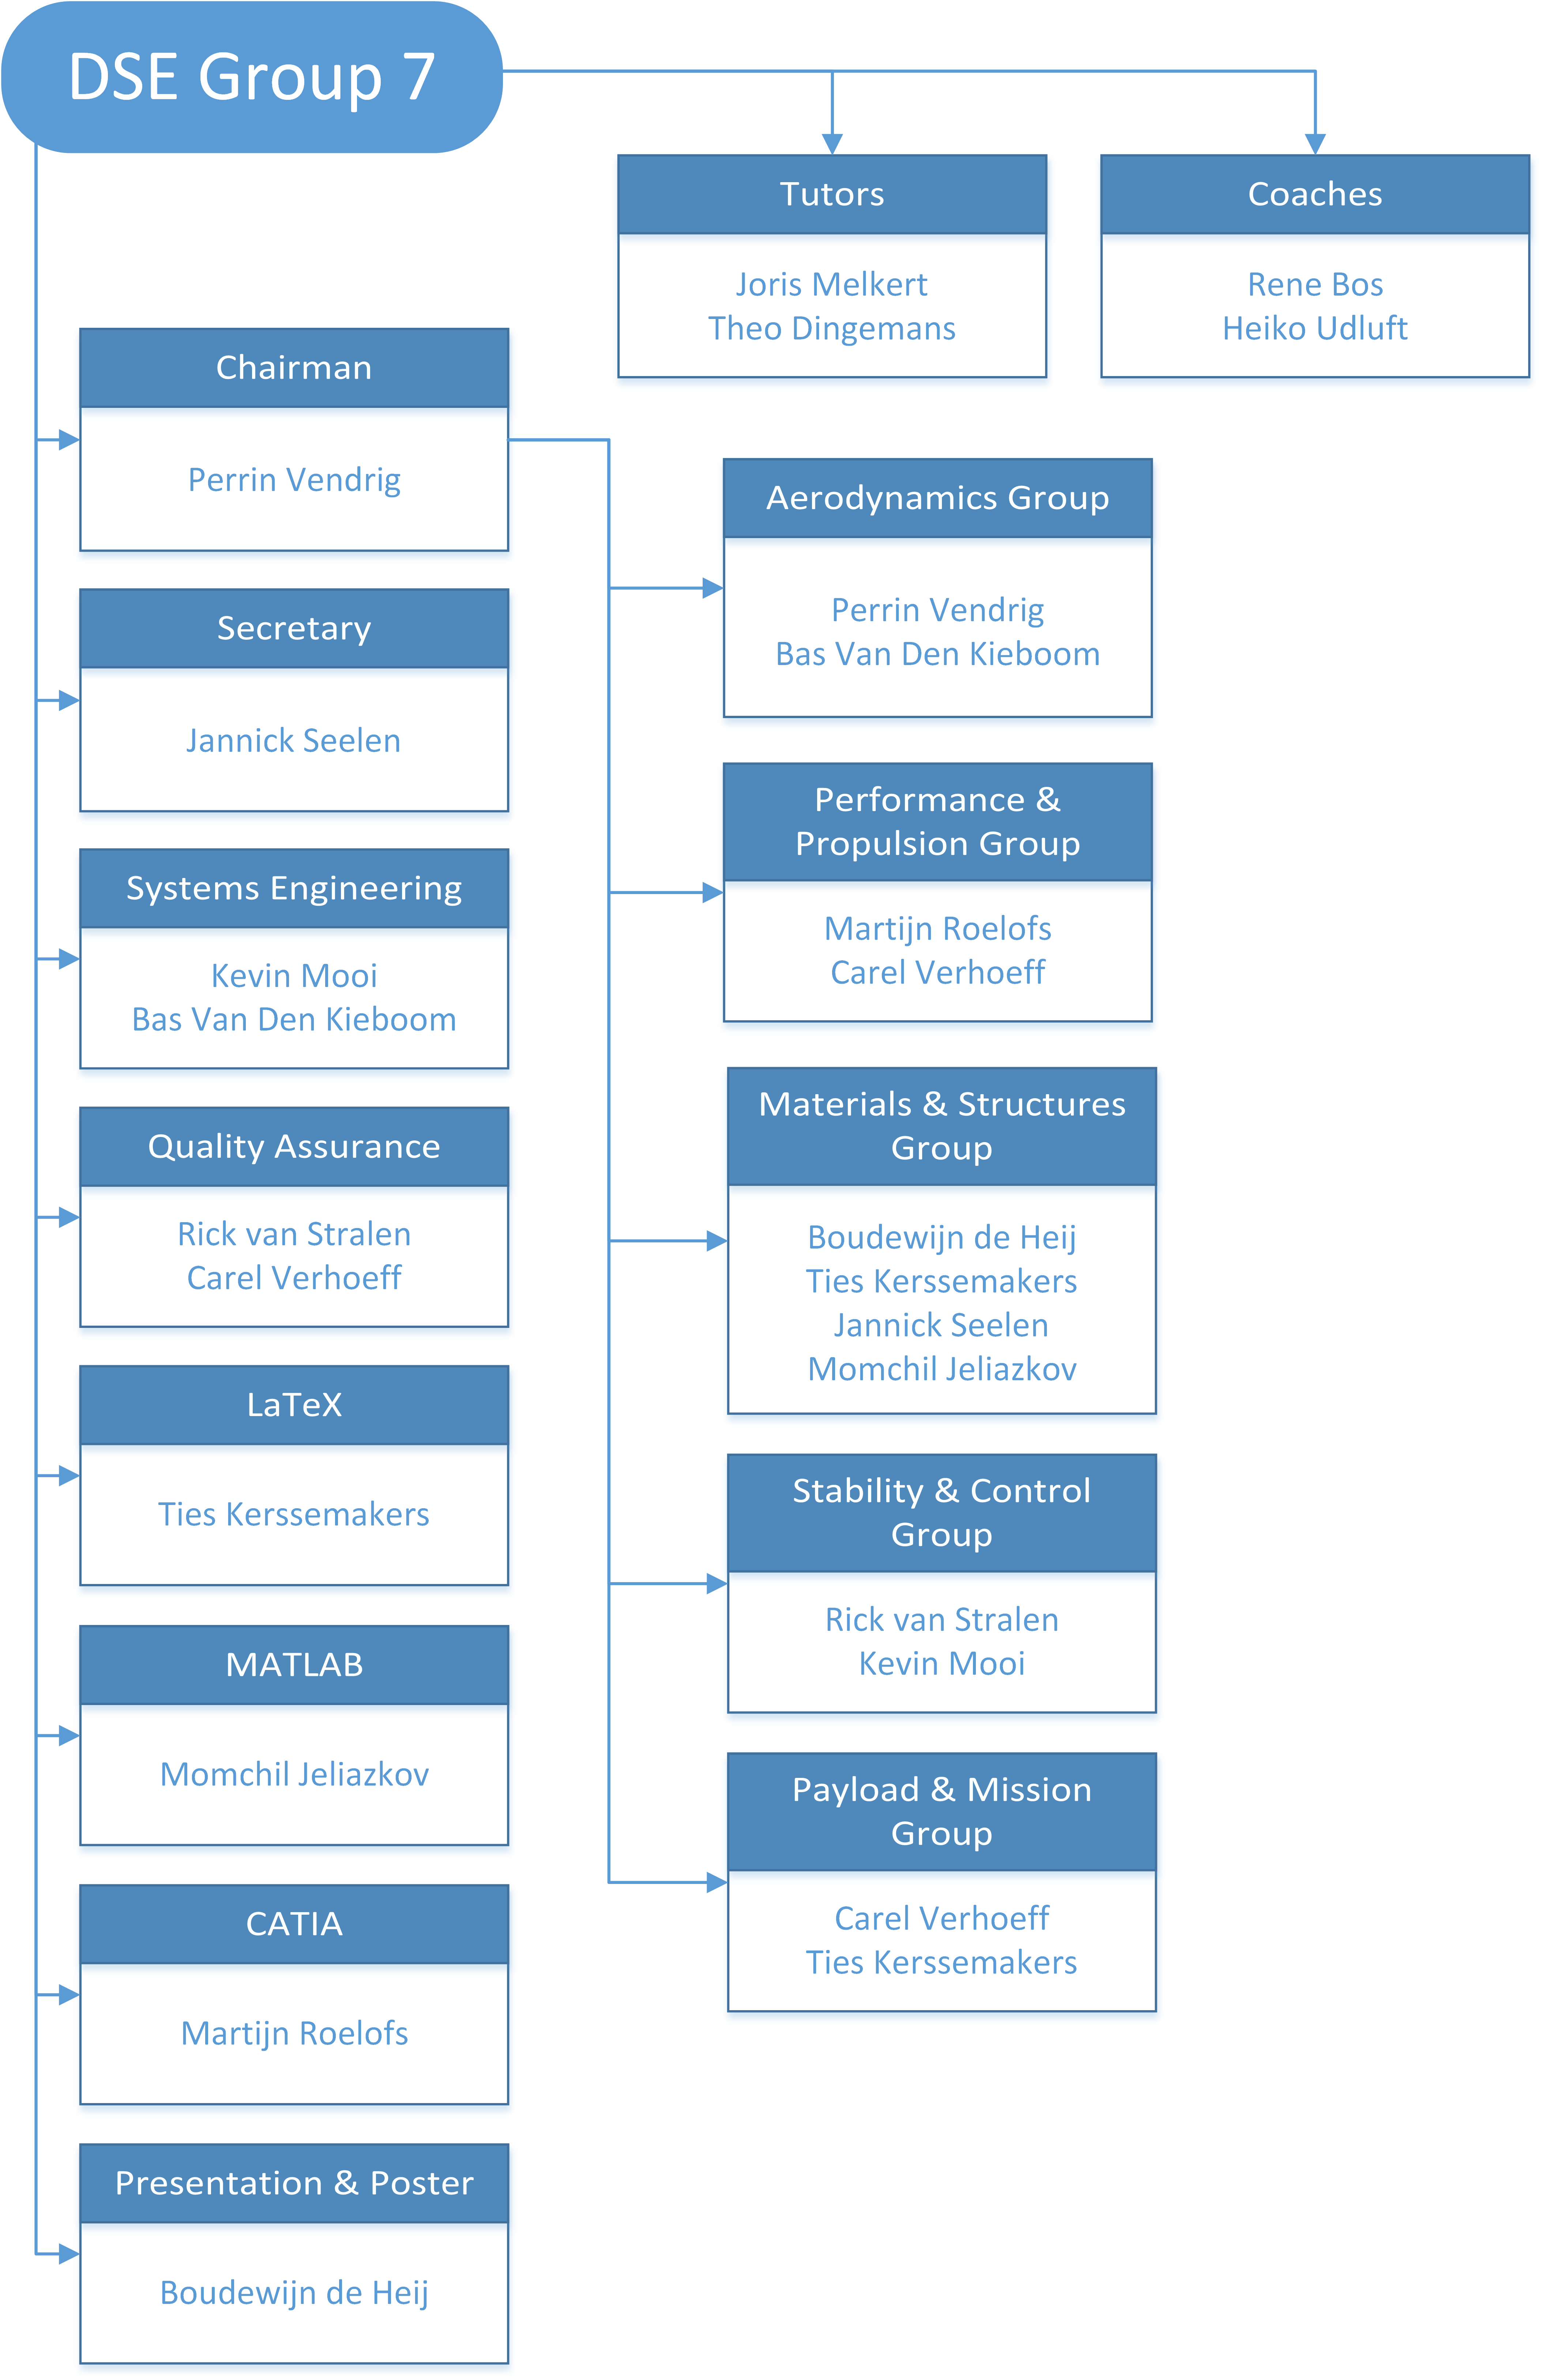
\includegraphics[width=0.6\textwidth]{Figures/Organogram2.png}
\caption{Organogram of the team organization}
\label{fig:Orgroles}
\end{figure}
\documentclass[a4paper]{report}
\usepackage[english]{babel}
\usepackage{amssymb}
\usepackage{amsmath}
\usepackage{graphicx}
\usepackage{float}
\usepackage{shortvrb}
\usepackage{cancel}
\usepackage[T1]{fontenc}
\usepackage{nicefrac}
\usepackage{amsfonts}
\usepackage{standalone} %Makes it possible to ignore other preambles of child document
\usepackage{eurosym} %Euro teken mogelijk
\usepackage{multirow} %For multiple rows togheter in one table
\usepackage{parskip} %For a small white line between paragraphs
\usepackage[protrusion=true,expansion=true]{microtype}
\usepackage{hyperref}%For automatic and URL Reference
\usepackage{appendix}
%Possible to change the margins
\usepackage{geometry}
\geometry{verbose,tmargin=1.9cm,bmargin=1.8cm,lmargin=2cm,rmargin=2cm}

\usepackage{subfig}

%include pdf pages
\usepackage{pdfpages}

%being able to create tables over multiple pages
\usepackage{longtable}

\makeatletter

%Change standard font size
\renewcommand\normalsize{ \@setfontsize\normalsize{11pt}{11pt}}\normalsize  
\makeatother

\usepackage{fancyhdr}
\pagestyle{fancy}
\fancyhead{}
\fancyfoot{}

%Gives text above each page
\fancyhead[CO,CE]{DSE Project}

%Page number
\fancyfoot[RO,LE]{\thepage}


\usepackage{babel}

%Available structures:
%Report: \part{}, \chapter{}, \section{}, \subsection{}, \subsubsection{}, \paragraph{}, \subparagraph{}


\begin{document}





\section{Control and monitoring the work}
To let the project run smoothly, some house rules and meetings are necessary. The house rules and meetings are needed to work as efficient as possible but also to create a good working environment. The house rules are:\\
\begin{itemize}
\item Follow the rules set by the DSE project and the Fellowship building.
\item Every day a logbook needs to be filled in by every member to specify what they did the past day during the working hours.
\item Every morning there is a brief meeting of 15 minutes.
\item Also weekly a meeting with the project mentors will be organized to give a status update and to have some time for questions from both students and mentors.
\item The working hours are from 9 am. till 5 pm.
\item Clean desk.
\item There is a lunch break of maximum 45 minutes each day.
\item When 15 minutes late one brings a cake next day.
\item Missing more than 2 hours at a particular day is considered a missed day.
\item All group stuff will be put in a locker at the end of the day.
\end{itemize}
The logbooks are needed to check what every member has been doing and if it takes too long to finish the part he is working on.\\
In the morning meetings a quick status update will be given and then is decided what should be done that day. During these meetings a status sheet will be filled in on how far the individual people are with their work. This status sheet will be filled in by the use of colours, green is the task is on schedule, yellow is a minor delay and red is a critical situation and the whole team must help. \\
The tutor meetings are needed to ask questions and to give a status update on how far the project has advanced. These meetings will take place once a week and the date will be planned with the tutors themselves. Before these meetings an agenda will be made to make the meeting as efficient as possible. The content of this agenda is determined during the weekly teammember meetings. At these weekly group meetings a summary will be made of the things that have been done so far.\\
If there is a delay by one of the group members or if deliverables can not be finished before the required deadlines, action should be taken. If one of the group members had an individual delay another group member can help or the one with the delay can finish it outside the project hour's. But if one of the deadlines is hard to complete the whole group should take action. These actions depend on the reason of the delay. The possible actions that can be taken are:
\begin{itemize}
\item Working outside the project hours.
\item Inform the tutors that it is impossible to deliver the report on time.
\item Decreasing the workload by leaving minor things out of the report and keep focus on the major issues.
\end{itemize}

\subsection{Version control}
Keeping track of changes and versions of project files is essential, especially for the reports, code files and CATIA. To keep this organized a SVN server is setup using virtualSVN server. A repository is installed on one team members' computer,  which acts as a server where the other members can update from and commit to. Using Version control programs such as tortoiseSVN on the client side makes it easy to commit one's changes and update the others'. Moreover, these tools provide merge options, to resolve possible conflicts. SVN has a changelog, in which each change is logged, with a message from the committer, the name of the committer, time/date and the affected files. The combination with the general logbook as well as the personal logbooks gives a clear view on the progress of the project. 
\end{document}


\end{document}